%% -*- mode: LaTeX; compile-command: "runhaskell Shake" -*-
\documentclass[xcolor=svgnames,12pt]{beamer}

\usepackage[all]{xy}
\usepackage{brent}
\usepackage[backend=cairo,outputdir=diagrams]{diagrams-latex}
\graphicspath{{images/}}

%%%%%%%%%%%%%%%%%%%%%%%%%%%%%%%%%%%%%%%%%%%%%%%%%%%%%%%%%%%%
%%%%%%%%%%%%%%%%%%%%%%%%%%%%%%%%%%%%%%%%%%%%%%%%%%%%%%%%%%%%

% Math typesetting

%%%%%%%%%%%%%%%%%%%%%%%%%%%%%%%%%%%%%%%%%%%%%%%%%%%%%%%%%%%%
%%%%%%%%%%%%%%%%%%%%%%%%%%%%%%%%%%%%%%%%%%%%%%%%%%%%%%%%%%%%

\newcommand{\theschool}{Williams College}
\newcommand{\thedate}{March 13, 2015}

%%%%%%%%%%%%%%%%%%%%%%%%%%%%%%%%%%%%%%%%%%%%%%%%%%%%%%%%%%%%
%%%%%%%%%%%%%%%%%%%%%%%%%%%%%%%%%%%%%%%%%%%%%%%%%%%%%%%%%%%%

\setbeamertemplate{items}[circle]

\mode<presentation>
{
  \usetheme{default}                          % use a default (plain) theme

  \setbeamertemplate{navigation symbols}{}    % don't show navigation
                                              % buttons along the
                                              % bottom
  \setbeamerfont{normal text}{family=\sffamily}

  % XX remove this before giving actual talk!
  % \setbeamertemplate{footline}[frame number]
  % {%
  %   \begin{beamercolorbox}{section in head/foot}
  %     \vskip2pt
  %     \hfill \insertframenumber
  %     \vskip2pt
  %   \end{beamercolorbox}
  % }

  \AtBeginSection[]
  {
    \begin{frame}<beamer>
      \frametitle{}

      \begin{center}
        \includegraphics[width=2in]{\sectionimg}
        \bigskip

        {\Huge \insertsectionhead}
      \end{center}
    \end{frame}
  }
}

\defbeamertemplate*{title page}{customized}[1][]
{
  \vbox{}
  \vfill
  \begin{centering}
    \begin{beamercolorbox}[sep=8pt,center,#1]{title}
      \usebeamerfont{title}\inserttitle\par%
      \ifx\insertsubtitle\@@empty%
      \else%
        \vskip0.25em%
        {\usebeamerfont{subtitle}\usebeamercolor[fg]{subtitle}\insertsubtitle\par}%
      \fi%
    \end{beamercolorbox}%
    \vskip1em\par
    {\usebeamercolor[fg]{titlegraphic}\inserttitlegraphic\par}
    \vskip1em\par
    \begin{beamercolorbox}[sep=8pt,center,#1]{author}
      \usebeamerfont{author}\insertauthor
    \end{beamercolorbox}
    \begin{beamercolorbox}[sep=8pt,center,#1]{institute}
      \usebeamerfont{institute}\insertinstitute
    \end{beamercolorbox}
    \begin{beamercolorbox}[sep=8pt,center,#1]{date}
      \usebeamerfont{date}\insertdate
    \end{beamercolorbox}
  \end{centering}
  \vfill
}

\newenvironment{xframe}[1][]
  {\begin{frame}[fragile,environment=xframe,#1]}
  {\end{frame}}

% uncomment me to get 4 slides per page for printing
% \usepackage{pgfpages}
% \pgfpagesuselayout{4 on 1}[uspaper, border shrink=5mm]

% \setbeameroption{show only notes}

\renewcommand{\emph}{\textbf}

\title{Polynomial Functors Constrained by Regular Expressions}
\date{\theschool \\ \thedate}
\author{Brent Yorgey}
\titlegraphic{XXX}

%%%%%%%%%%%%%%%%%%%%%%%%%%%%%%%%%%%%%%%%%%%%%%%%%%%%%%%%%%%%

\begin{document}

\begin{xframe}{}
   \titlepage
   %% XXX picture of dissected tree from paper
%   \hfill \includegraphics[width=0.5in]{plclub}
\end{xframe}

%%% Fun to be here.  Work I do is at the intersection of math & CS.
%%% Please ask questions!  Part of my challenge is to translate some
%%% CS things for mathematicians and vice versa.

%%% First two parts: get you to understand title, i.e. problem
%%% statement.  Part 3: our solution.  Based on joint work with Dan
%%% Piponi.

\begin{xframe}
  \begin{center}
    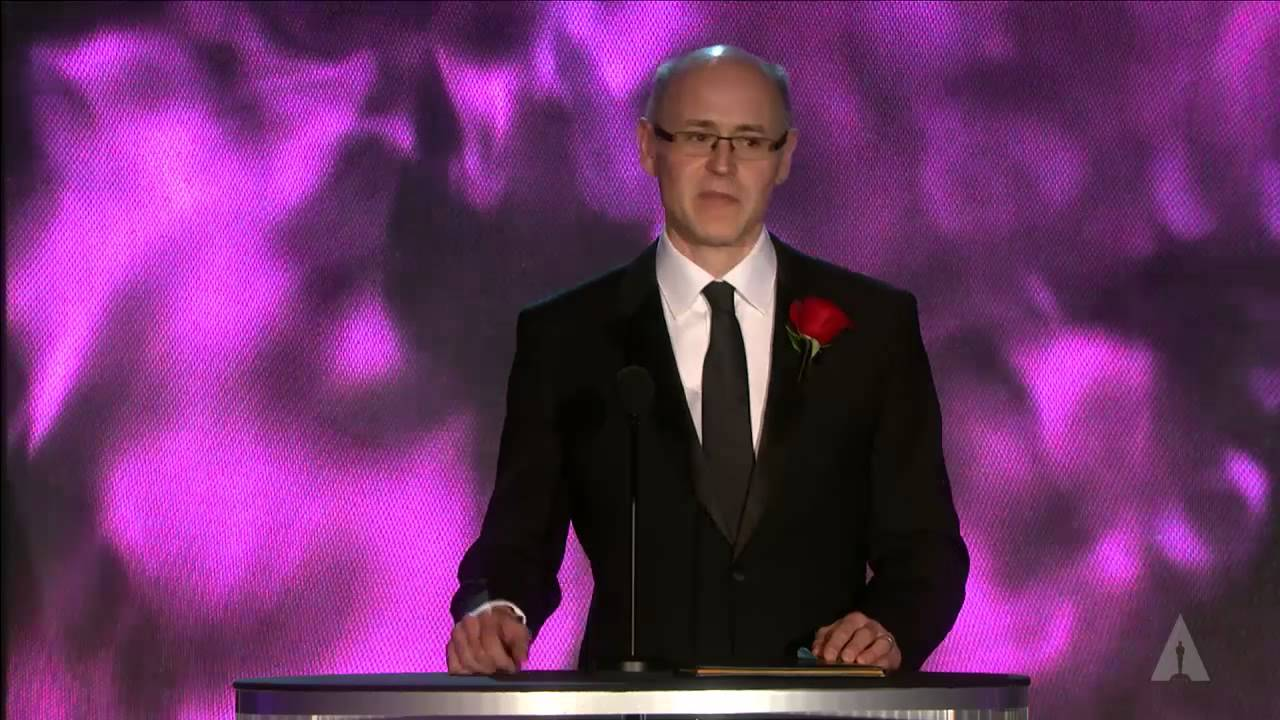
\includegraphics[width=2in]{dan}

    Joint work with Dan Piponi
  \end{center}
\end{xframe}

\def\sectionimg{dan.jpg}
\section{Polynomial functors}

\begin{xframe}{Polynomial functors}
  \begin{center}
  \[ F : \Set \to \Set \]

  XXX picture here of a set of elements being sent to set of
  structures built from them.

  \emph{(parameterized) combinatorial families}
  \end{center}
\end{xframe}

\begin{xframe}{Building polynomial functors}
  Polynomial functors are those $F : \Set \to \Set$ which can be built
  up out of:
  \begin{align*}
    0(A) &= \varnothing \\
    1(A) &= \{\star\} \\
    X(A) &= A \\
    (F + G)(A) &= F(A) \uplus G(A) \\
    (F \cdot G)(A) &= F(A) \times G(A)
  \end{align*}
\end{xframe}

\begin{xframe}{Example}
  \begin{gather*}
    1 + ((X \cdot X) + X) : \Set \to \Set \\
    (1 + ((X \cdot X) + X))(A) = \{\star\} \uplus ((A \times A) \uplus A)
  \end{gather*}
\end{xframe}

\begin{xframe}{Polynomial functor isomorphisms}
  Note that
  \begin{gather*}
    F + (G + H) \cong (F + G) + H \\
    0 + F \cong F \cong F + 0 \\
    F \cdot (G \cdot H) \cong (F \cdot G) \cdot H \\
    1 \cdot F \cong F \cong F \cdot 1
  \end{gather*}
\end{xframe}

\begin{xframe}{Polynomial functor isomorphisms}
\[ 1 \cdot F \cong F \cong F \cdot 1 \]

Example proof:

  \begin{align*}
    (1 \cdot F)(A) &= 1(A) \times F(A) \\
    &= \{\star\} \times F(A) \\
    &= \{(\star, f) \mid f \in F(A)\} \\
    &\cong F(A).
  \end{align*}
\end{xframe}

\begin{xframe}{Implicit/recursive definition}
  XXX also allow implicit/recursive definitions
\end{xframe}

\begin{xframe}{Example: binary trees}
  XXX Example: binary trees
  (show Haskell)
\end{xframe}

\begin{xframe}{Example: even/odd lists}
  XXX example: even/odd lists
\end{xframe}

\begin{xframe}{``Polynomial''?}
  
\end{xframe}

\end{document}